\chapter{调制识别的深度学习框架探索}
\section{引言}
我们将深度神经网络应用到无线电调制识别任务中,研究机器学习的最新进展。 结果表明,无线电调制识别不受网络深度的限制,进一步的工作应着重于提高学习的同步和均衡。 这些领域的进步可能来自为这些任务设计的新架构或通过新颖的培训方法。\par

在将深度神经网络应用于无线通信信号之前,值得回顾其他应用领域的现状。下一节将回顾深度神经网络架构和学习进展,这些进展可能对无线通信应用是有效的和有用的。在回顾有趣的深层架构和训练方法之后,结果在第三部分和第四部分讨论。 \par

\subsection{卷积神经网络}
在所有现有技术的深度神经网络中的共同元素是卷积层的使用。卷积层由Nf个卷积滤波器组成。图像和手写识别开始使用卷积图层来提供特征平移不变性[8]。神经网络中卷积滤波器的使用可能与已经熟悉FIR滤波器和DSP的人员的预期略有不同,至少部分是由于在神经网络中使用激活函数。神经网络中的卷积通常非常小(1x1到5x5是图像处理中的常见尺寸)。在典型的DSP应用中,滤波器非常宽(很多抽头/高阶)而不是深(小抽头,但是级联)。实现这些滤波器的现代方法(诸如多相滤波器组)通常提供了用于计算或等待时间原因来减小滤波器宽度的方法。标准卷积层[9]的传递函数在下面的等式3中给出,其中yi是第i个滤波器的输出特征图,b和k表示学习偏差和滤波器权重参数,xi表示输入激活,*表示卷积运算,并且f(..)表示诸如整流线性单元(ReLU)或S形的(通常非线性的)激活函数。\par

图像处理的神经网络的一个明显的趋势是建立更深的网络,以学习更复杂的功能和层次特征关系[2],[1]。深度网络使得更复杂的功能可以从原始数据中更容易地学习,而不是更浅的网络,具有相同数量的参数[1],[18]。然而,人们普遍认为,神经网络中的深度受到不稳定梯度的限制,不稳定梯度在网络中的早期层或后一层爆炸或消失。
近年来,通过在优化器中使用梯度归一化以及不会加剧消失梯度问题的非线性(如整流线性单位(ReLU)),这个问题已经得到改善。结果,几个重要的架构已经被用来通过增加深度来赢得竞争,比如ImageNet,我们将会考虑改善无线电调制识别。\par

\subsection{GoogLenet}
GoogLenet [17]中使用的初始体系结构是增加网络深度的一个成功方法,能够在不同尺度的特征上推广,同时仍然管理复杂性。这个网络由重复的启动模块组成。每个启动模块(如图1所示)包含四条并行路径,输出是四个并行输出的串联。第一条路径是沿选定信息转发的1×1卷积的银行。 1x1卷积是一种选择性高速公路网络,它只是简单地向前传递信息而不进行变换。第二和第三路径是1×1卷积,接着是一组3×3和5×5卷积以提供多个比例的特征检测。最后,最后一个并行路径是一个3x3共享层,然后是1x1卷积。网络中的中间启动模块连接到softmax分类器,导致网络全球培训损失。这些分类器被认为有助于防止消失梯度。另一种增加深度的方法是使用架构来跨层转发信息。到目前为止,赢得ImageNet 2015最好的方法是残余网络[4]。剩余网络将一层的输出添加到更深层的输出层(如图2所示)。这就是所谓的残差网络,因为转发的信息迫使网络学习一个残差函数,如图1:从[17]中的初始单元图,推广到多尺度的特征学习,同时也管理模型的复杂性。\par

图2:来自[4]的剩余网络图,允许来自多个源层的特征映射组合选择网络内的最佳架构路径。部分特征提取。剩余网络作者认为消失梯度可以通过已被广泛采用的规范化技术来解决,网络深度反而受限于深度网络的训练复杂度,可以用残差函数简化。\par


\subsection{CLDNN}
CLDNN是语音处理的一种方法,它在原始的时域波形上运行,而不是像log-mel cepstrums [16],[15]这样的专家语音功能。该体系结构使用两个卷积层,然后是两个递归层
由长期短期记忆(LSTM)单元组成。 LSTM是一个常见的经常性网络架构,由几个门控制,历史维持多久[5]。 CLDNN也可以具有绕过层的连接,这些层旨在为提取的功能提供更长的时间上下文。例如,原始CLDNN在LSTM层之前转发具有卷积层输出的原始样本[15]。\par

受到使用专业知识指导网络体系结构(如卷积网络和CLDNN)的启发,我们尝试使用卷积网络,我们将其称为卷积匹配滤波器。相当简单的想法是采用典型通信接收机的通用架构,并构建具有相似部分的神经网络架构。通信接收机有一个滤波器(通常与传输的脉冲或波形匹配),同步器和采样器。通常,前置滤波器抽取每个符号的少量采样,用于执行相移以找到最佳采样点的同步器。采样器然后切片到比特或者发出用于模拟调制的音频。与此类似的神经网络体系结构是一个卷积层,随后是一个LSTM。\par


\section{不同框架的识别性能}

\subsection{神经网络训练}

网络的超参数(如学习速率,每层过滤器/特征映射的数量,过滤器的大小以及层的数量)都会影响网络规模,难以优化。最近的研究尝试将超参数优化为可以用反向传播和梯度下降(如网络权重和偏差)进行训练的常规参数。对于这项研究,我们忽略训练超参数,并使用adam优化器[6],它提供了梯度归一化和动量,降低了像学习率这样的超参数的重要性。在工作的指导下,深度比特征图的数量更重要[2],我们将建立一个类似于无线电卷积调制网络[13]中使用的基线卷积网络。我们的第一步是调整每个滤波器的滤波器数量和抽头数量,并将其视为不重要的超参数,用于剩余的实验,以测试不同架构对RF数据的适用性。\par

我们使用RadioML2016.10a数据集[12]作为评估调制识别任务的基础。目标是使用128个样本的复合(基带I / Q)时域矢量来识别11种可能类别中的调制方案。 128个样本以2x128向量馈入网络,其中复数时间样本的实部和虚部被分开。该数据集使用功率延迟分布,频率选择性衰落,本地振荡器偏移和加性高斯白噪声以及这些效应的细节[12]。数据集标有调制类型和SNR地面实况。我们使用全信噪比top-1分类精度作为单一数字基准,并且比较技术显示SNR高于1的精度。\par

所有模型和培训都是通过使用Nano GTX 1070 GPU的theano后端Keras深度学习库完成的。我们从一个类似于CNN2网络的网络开始[13]。这是选择的基线,因为[13]的结果显示专家方法的显着改善;任何进一步的改进应被认为是现有技术。主要区别在于我们将在每个图层上使用大小为1xtaps的滤镜。我们将做一个简单的超参数优化\par

•为RF调制识别找到最佳的滤波器数量和滤波器大小图3:改变每层滤波器的数量具有较小的影响,在较高的SNR下更明显。每个网络在2个卷积层网络中都有1×3的过滤器,有1个致密层和一个softmax分类器。\par

•测试从网络深度和过滤器大小的其他领域获得的假设\par

\subsection{基准卷积网络}

基线卷积网络在softmax分类器之前有两个卷积层和一个致密层。每个隐藏层具有整流线性单元(ReLU)激活功能和50%的丢失。第一个超参数优化是卷积层的大小。每个图层都有1x3的过滤器,我们将改变过滤器的数量来找出需要的数量。从[1],[18],[2]我们预计在过拟合发生之前,过滤器数量的大范围将会给出类似的性能。\par
\begin{figure}[!h]
	\centering
	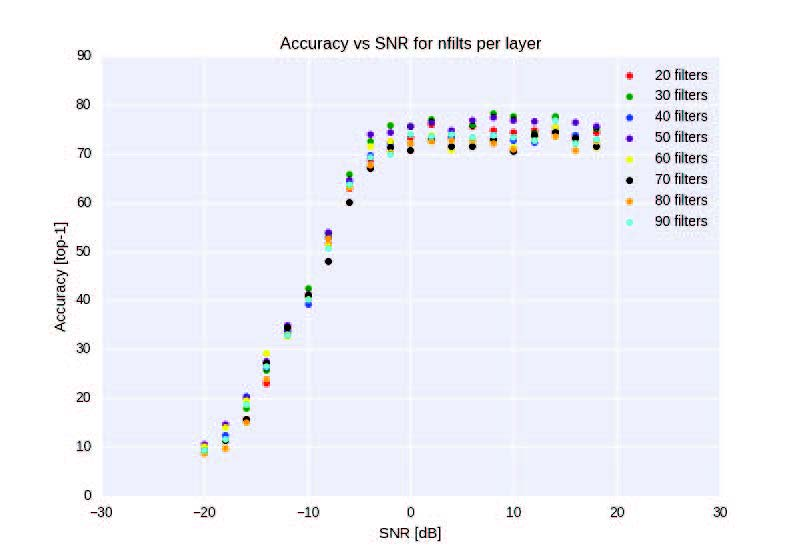
\includegraphics[scale=1]{figures/chapter_5/fig1}
	\caption{图阿斯顿发送到发送}\label{fig_5_1}
\end{figure}
正如所预料的那样,每层大约有30到70个过滤器,而且性能非常相似,这个过滤窗口相当大。对于10-滤波器增量,20-90滤波器的前1分类精度如图1所示。对于其余的实验,我们将使用每层50个滤波器。\par

接下来,我们优化每个过滤器的大小。[2]表明,滤波器的大小也有最小的影响,但基于无线电领域和数据集的专业知识,我们期望8-抽头滤波器是最佳的。对于这个实验,我们使用一个具有单隐藏密集层的双卷积层网络,接着是softmax分类器。卷积层每个都有50个滤波器,其滤波器大小为1xntaps,其中ntaps在3到12之间变化。每个卷积层的滤波器尺寸变化的结果表明,较小的滤波器不如较大的滤波器。我们根据数据集的专家知识假设8抽头滤波器是最好的。图2中每个信噪比图的结果很难区分清楚的赢家;然而,整个数据集分类准确性表明,7-12轻敲都有相似的性能约61%,差异在统计上不显着。\par
\begin{figure}[!h]
	\centering
	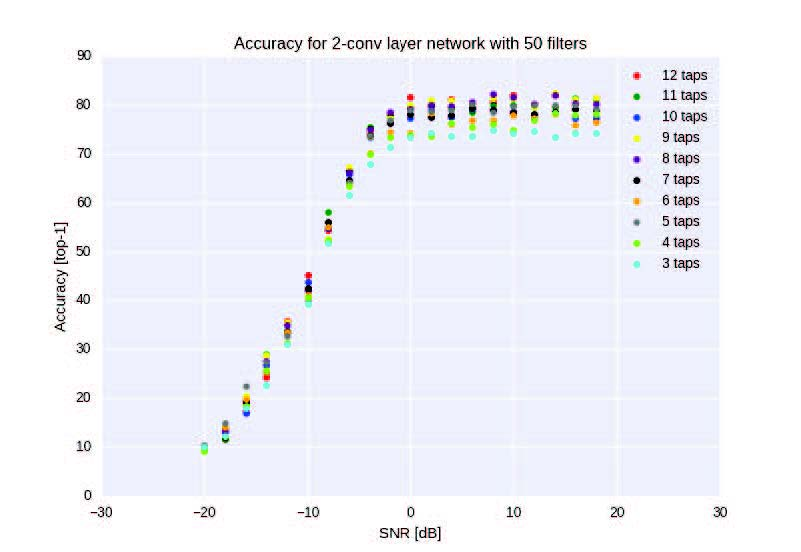
\includegraphics[scale=1]{figures/chapter_5/fig2}
	\caption{改变两个卷积层中的抽头数量(滤波器大小)。水龙头的数量明显较少,但是水龙头的数量增加}\label{fig_5_2}
\end{figure}
最后,对于纯卷积网络,我们尝试增加网络深度。对于这个实验,我们使用1x8滤波器的50抽头卷积层。卷积层之后,我们使用一个隐藏的密集层,然后是最后一个密集的softmax分类器。我们从一个2卷积层网络开始,并添加卷积层。深度学习的趋势表明,增加更多的层次应该改善分类性能,直到梯度变得不稳定。\par
改变卷积层的数目显示很少分类精度没有提高。这个任务的信噪比精度如图3所示。这表明我们的网络没有更多的特征深度学习。由于调制数据通常只改变复数正弦曲线的幅度,频率或相位,所以数据的起始层次不高。然而,增加更多的卷积层似乎并不能在较低的信噪比下帮助降低噪声的影响。图6:显示超参数优化的CNN和9层残留网络的训练损失和验证损失的训练历史记录。这两个网络导致类似的验证损失和训练损失,但剩余的网络在较少的时期训练。\par
\begin{figure}[!h]
	\centering
	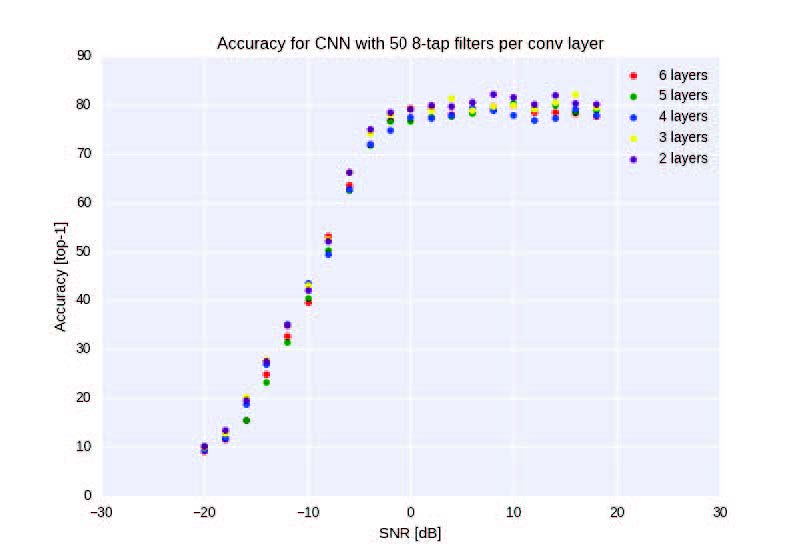
\includegraphics[scale=1]{figures/chapter_5/fig3}
	\caption{改变DNN中的卷积层的数量不会改进无线电调制识别。}
\end{figure}

\subsection{残留网络}

虽然增加更多的卷积层不会提高分类准确性并不奇怪,但令人惊讶的是,分类和丢失只要2或3个卷积层即可达到平坦。最初的重点是深层网络导致更高的训练损失,这表明更高的训练难度,而不是过度训练。图6显示,我们的超参数优化CNN和9层残留网络达到了相似的损失,验证损失和准确性没有显示;然而,残留网络学习的时间较少。我们还尝试了5-9层的残留网络,这些网络都具有相似的性能和训练时间。这与我们对于普通CNN深度的超参数搜索相结合,表明我们不受无线电学习任务的网络深度限制,尽管我们受到纯粹CNN架构可以学习的特征的限制。\par

\subsection{初始模块}

先启模块在我们的实验中也没有改进无线电调制分类,使用为我们的数据集调整的初始模块。每个模块使用的三个分支是50个1x1滤波器,50个1x3滤波器和50个1x8滤波器。\par
1x3和1x5滤波器分支前面也有50个1x1滤波器,如图7所示。网络中1-4个初始模块的结果没有显示出超过我们的超参数优化CNN的改进。同样,这表明我们不受深度的限制,也不受限于过滤器的规模。\par

\subsection{LSTM网络}

作为我们测试的最终架构,增加了经常性的网络层,即由LSTM单元组成的层,用于对时间特征进行建模。这种方法在时间序列应用中被广泛使用,我们预计调制基带时间序列可能同样适用。我们测试了两层和三层卷积,然后在CLDNNtype体系结构中使用循环层,在循环层之前有和没有正向/旁路连接。我们发现如图8所示的前向连接作为原始波形和卷积输出的连接,导致比其他体系结构更好的分类精度和更稳定的梯度下降。使用会创建类似前面描述的卷积匹配滤波器检测器的结构的合并层不利于分类。\par

为了进一步理解什么限制了分类的准确性,我们看一下图10所示的CLDNN的混淆矩阵。有两个主要的混淆领域。一个在模拟调制之间,另一个在高阶QAM之间。模拟调制将很难解决,但是QAM可以在更好的同步和减少信道损伤的情况下得到改善。对CLDNN在每一层学习的内容有直观的认识,对于指导未来的工作很重要。为此,我们绘制了一些滤波器抽头的时间和频率表示。对于频率响应,滤波器抽头用100个零填充以获得128点FFT。图图11a和12a示出来自第一层的两个选择滤波器。专家的眼睛看起来并不特别熟悉时域表示;然而频率响应确实显示了成形的低通滤波器。未示出的其他滤波器具有频率选择性组件,DC阻断器和类似sinc的频谱形状。\par

将这些滤波器可视化的另一种方法是将随机数据应用于它们,并对特定滤波器的输出执行梯度上升,该滤波器将收敛于最能激活卷积神经元的数据上[11]。选定的两个过滤器的结果如图所示。由此产生的载体看起来有点像粗PSK和FM / FSK调制到专家的眼睛。由于模拟的信道模型,矢量也显示出我们的数据集中存在的一些恒定的相位旋转。需要注意的是,选择这两个过滤器可视化并不是所有的过滤器都对专家有意义。\par


\section{结果及分析}

\section{本章小结}
深度神经网络在无线电领域的性能似乎不受网络深度的限制,就像图像,自然语言处理和声学领域一样。 尽管我们的实验将调制识别作为基准任务,但是我们期望其他无线机器学习任务能够使用类似的网络架构。 无线电任务深度学习的进一步发展可能来自改进的训练方法和网络架构,这些架构可以学习转换射频数据以消除无线信道的影响,这种神经网络架构不是为此设计的。 目前正在探索的一个例子是使用空间变换来均衡和同步输入波形[14]。